\documentclass[10pt,twocolumn]{article}

\usepackage[letterpaper,margin=1in,columnsep=0.25in]{geometry}
\usepackage[T1]{fontenc}
\usepackage{lmodern}
\usepackage{microtype}
\usepackage{amsmath,amssymb}
\usepackage{booktabs}
\usepackage{array}
\usepackage{enumitem}
\usepackage{tabularx}
\usepackage{tikz}
\usepackage{url}
\usepackage[hidelinks]{hyperref}

\hypersetup{
  pdftitle={Fail-Closed Evidence for Decision-Fidelity Evaluation of Collective Trace Replay},
  pdfauthor={Anshuman Agrawal},
  pdfkeywords={collective communication, trace replay, decision fidelity, reproducibility, NCCL}
}

\setlist{nosep,leftmargin=*}
\raggedbottom
\newcommand{\wname}[1]{\texttt{W-#1}}
\newcommand{\us}{\,\mu\mathrm{s}}
\newcolumntype{L}[1]{>{\raggedright\arraybackslash}p{#1}}
\newcolumntype{Y}{>{\raggedright\arraybackslash}X}

\title{Fail-Closed Evidence for Decision-Fidelity Evaluation\\
  of Collective Trace Replay}
\author{Anshuman Agrawal\\
  \small CommCanary Project\\
  \small\url{https://github.com/iemAnshuman/CommCanary}}
\date{}

\begin{document}
\maketitle

\begin{abstract}
Collective communication traces let researchers study distributed workloads
without rerunning the full application, but replaying the recorded calls does
not guarantee the same configuration choice. CommCanary provides a fail-closed
workflow for freezing, selecting, archiving, and independently checking collective-trace
replay evidence. Its publication path binds a campaign to immutable attempts,
an explicit selection, a completeness verdict, a hash-identified archive, and
deterministic analysis. The workflow withholds claims when required evidence
is missing or fails the declared stability policy.

We compare four proxy representations with a full workload on one node with
four NVIDIA A100 GPUs and eight NCCL configurations. The trusted join contains
all 280 selected cells. Communication-only replay does not preserve the
measured configuration ranking: \wname{canary} agrees on 16 of 28 pairs, with
a 95\% repetition-bootstrap interval of 12 to 17. It ranks the full
workload's slowest configuration second. Replay that keeps compute concurrent
with communication places both low-latency-protocol configurations where the
full workload does, and \wname{shared-overlap} agrees on 20 pairs, more
than \wname{canary} in 99.9\% of bootstrap draws. These differences depend on
one configuration, \texttt{nccl-2.20.5-tree-ll}. After excluding it, the
reported pair-agreement difference intervals all include zero.

A retrospective decision-regret analysis measures the cost of each proxy's
first choice on the full workload. Communication-only replay and the
microbenchmark both incur 3.16\% point regret; configuration-specific overlap
replay chooses the measured optimum despite having the lowest pair agreement.

A separate exact-work gate reports 26 of 28 agreeing pairs, or 92.86\%, with
$\tau_b=0.857$, one false negative, one false positive, 1.55\% median absolute
relative error, and 4.05\% p95 error. The persisted verdict is
\emph{inconclusive}, not pass. Bootstrap intervals cross frozen decision
boundaries, and one configuration exceeds the relative-IQR stability limit.
The evidence supports a measured negative result about communication-only
replay and an independently verifiable publication workflow. It does not
qualify CommCanary as a production gate, prove general decision preservation,
or establish savings from a reduced physical canary.
\end{abstract}

\section{Introduction}

Distributed machine learning and high-performance computing systems often
require a choice among collective algorithms, protocols, or library versions.
That choice depends on more than message size. Process arrival times, network
topology, endpoint resource use, operation order, and overlap with computation
can all change the ranking. MPI implementations therefore select among
multiple collective algorithms, and NCCL exposes algorithm and protocol
choices whose performance depends on workload context~\cite{mpi,nccl,thakur,vadhiyar}.
An isolated microbenchmark can measure a collective precisely while omitting
the execution conditions that determine the application choice.

Execution traces provide another way to study a workload. A trace can record
operations and dependencies; a simulator or replay engine can then execute the
recorded structure without rerunning the original application
\cite{chakra,mystique,astrasim,astrasim2,scalatrace,loggopsim}. The tuning
question is whether replay selects the same configuration as the full
workload. Small timing error is not enough if replay
reverses two close configurations. High point agreement is also insufficient
when the measurements are unstable or uncertainty spans the decision boundary.

This work asks whether collective-trace replay preserves the pairwise
configuration decisions of a full workload, and whether the evidence path
refuses a positive claim when completeness, uncertainty, or stability is
inadequate.

CommCanary freezes each campaign before execution and retains every attempt
as an immutable record. An explicit selection identifies one terminal attempt
for each expected cell; a completeness verdict checks that the selected matrix
is present, unambiguous, and successful. The workflow then archives and hashes
the raw evidence and generates publication files deterministically from the
selection. Analysis stops if a required check fails.

We use this workflow in two experiments. The first joins three complete
campaigns into 280 selected cells covering eight NCCL configurations and seven
workload profiles. It compares four proxy representations with the full
workload. Communication-only \wname{canary} agrees on 16 of 28 configuration
pairs, or 57.1\%. Isolated \wname{micro} agrees on 18, or 64.3\%. A shared trace
replay with concurrent compute reaches 20, or 71.4\%. No proxy preserves all
decisions. We report repetition-bootstrap intervals for every count and a
sensitivity analysis that removes the one configuration driving the
differences between proxies.

The second experiment reconstructs the source-derived work exactly and
evaluates it with a policy frozen before analysis. Exact work reaches 26 of 28
pair agreement with low relative timing error. Every point criterion passes.
The gate still returns inconclusive because pair intervals cross tie boundaries
and the \texttt{nccl-2.20.5-tree-ll} configuration is unstable in three
representations. The reported point estimates therefore do not qualify exact
work under the frozen policy.

The paper contributes four items:

\begin{enumerate}
  \item a fail-closed evidence model for physical collective-replay experiments,
    with immutable attempts, explicit selection, completeness, archive binding,
    and deterministic publication;
  \item a complete 280-cell comparison showing that communication-only replay
    does not preserve the measured ranking. Uncertainty and sensitivity
    analyses bound this result, and retrospective decision regret measures
    the cost of the selected configuration separately from pair agreement;
  \item a predeclared exact-work gate whose point criteria pass but whose
    final verdict remains inconclusive; and
  \item an implementation of trace-bound candidate construction and physical
    gating, with its software contracts separated from the physical evidence
    needed to qualify a reduced canary.
\end{enumerate}

All physical observations come from a single node with four A100 GPUs. The
results do not establish multi-node behavior, expert-parallel replay,
congestion fidelity, CUDA-graph fidelity, vendor qualification, production-CI
readiness, or runtime savings from a reduced canary.

\section{Problem definition}

\subsection{Configuration depends on context}

Collective operations define group communication semantics while leaving
implementation strategy open~\cite{mpi}. Classic MPI work shows that no single
algorithm dominates across message sizes, process counts, and systems
\cite{thakur,vadhiyar}. NCCL provides topology-aware GPU collectives and allows
algorithm and protocol selection~\cite{nccl}. Our configuration set contains
two NCCL versions at default selection and six choices formed by crossing Ring
or Tree with LL, LL128, or Simple on NCCL 2.20.5.

An isolated microbenchmark is useful for transport characterization and
regression isolation. It intentionally removes application context. Concurrent
compute and communication can contend for endpoint resources and change the
critical path~\cite{overlap}. Arrival skew, explicit waits, dependencies, and
buffer lifetimes can also change which configuration is preferred. The
microbenchmark ranking must therefore be checked against the full workload
before it is used for configuration selection.

\subsection{Trace replay and surrogates}

Trace systems support different goals. ScalaTrace compresses and replays
communication traces~\cite{scalatrace}. LogGOPSim combines traces with an
analytical communication model~\cite{loggopsim}. ASTRA-SIM explores distributed
training systems through workload and network models~\cite{astrasim,astrasim2}.
Chakra defines an execution-trace schema for operations and dependencies,
while Mystique derives portable AI benchmarks from execution traces
\cite{chakra,mystique}. PARAM supplies communication benchmark and replay
tooling used by the experiment path~\cite{param}.

CommCanary uses existing trace formats and replay machinery to test decision
fidelity: whether a replay supports the same configuration choice as the source
workload under a frozen policy. The evaluation requires complete physical
evidence and can withhold a qualification claim even when a replay executes
successfully.

\subsection{Decision fidelity}
\label{sec:fidelity}

Let $C$ be the measured configurations and $R$ a representation such as the
full workload, a microbenchmark, or a replay. For each unordered pair $(a,b)$,
a policy maps timing distributions to
\begin{equation}
  d_R(a,b) \in \{a \prec b,\; a \sim b,\; b \prec a\},
\end{equation}
where $\prec$ means faster and $\sim$ means an operational tie. Agreement
between representation $R$ and the full workload $F$ is
\begin{equation}
  A(R,F)=\binom{|C|}{2}^{-1}\sum_{a<b}
  \mathbf{1}[d_R(a,b)=d_F(a,b)].
\end{equation}

Eight configurations produce 28 pair decisions. We also report Kendall's
tie-adjusted statistic~\cite{kendall}:
\begin{equation}
  \tau_b=\frac{N_c-N_d}
  {\sqrt{(N_c+N_d+T_R)(N_c+N_d+T_F)}}.
\end{equation}
Here $N_c$ and $N_d$ count concordant and discordant pairs, while $T_R$ and
$T_F$ count pairs tied on only one side. Exact agreement requires the same
three-way label. Kendall $\tau_b$ discounts some tie disagreements. Reporting
both exposes cases where a representation preserves the non-tied order but
changes many decisions into ties.

The trusted join uses its analyzer's frozen IQR rule. A pair is tied when its
median difference is smaller than either configuration's IQR. The exact-work
gate is a separate experiment with a pair-specific tie band, bootstrap
intervals, and a stability requirement. Its thresholds are not applied
retroactively to the trusted join.

\subsection{Point estimates and verdicts}

Performance samples can be autocorrelated, multimodal, or sensitive to machine
state. Scientific benchmarking practice calls for a complete method, repeated
observations, and explicit uncertainty~\cite{benchmarking}. The exact-work gate
uses percentile-bootstrap intervals~\cite{efron} and a relative-IQR stability
limit. A point estimate can pass while its interval overlaps a tie or reversal
region. The policy then returns insufficient evidence instead of pass.

\section{CommCanary evidence model}

\subsection{Fail-closed publication path}

Figure~\ref{fig:path} shows how the publication path checks campaign identity,
measurement completeness, and the provenance of the reported results.

\begin{enumerate}
  \item The campaign manifest freezes the matrix, environment identities,
    producer identities, policies, and expected cells before measurement.
  \item Each cell owns an immutable sequence of attempts. A retry appends a new
    attempt.
  \item A selection names the terminal attempt used for every expected cell
    and is itself hashed.
  \item A completeness verdict checks cardinality, identity, terminal status,
    and declared artifacts.
  \item An archive descriptor binds the retained raw evidence to exact bytes.
  \item The analyzer emits aggregate JSON and CSV, a paper fragment, and policy
    verdicts from the selected evidence.
\end{enumerate}

Aggregation requires a persisted completeness verdict, even when a parser can
compute a number from the available samples. Synthetic fixtures test software
behavior and are excluded from physical results. Operational notes may explain
an attempt, but cannot replace an aggregate or persisted verdict.

\begin{figure*}[t]
  \centering
  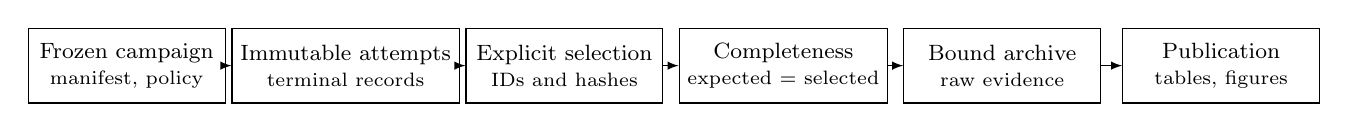
\begin{tikzpicture}[x=1cm,y=1cm,>=latex,font=\footnotesize,
  stage/.style={draw,minimum width=2.5cm,minimum height=0.95cm,align=center,inner sep=3pt}]
\node[stage] (s0) at (0.00,0) {Frozen campaign\\{\scriptsize manifest, policy}};
\node[stage] (s1) at (2.78,0) {Immutable attempts\\{\scriptsize terminal records}};
\node[stage] (s2) at (5.56,0) {Explicit selection\\{\scriptsize IDs and hashes}};
\node[stage] (s3) at (8.34,0) {Completeness\\{\scriptsize expected = selected}};
\node[stage] (s4) at (11.12,0) {Bound archive\\{\scriptsize raw evidence}};
\node[stage] (s5) at (13.90,0) {Publication\\{\scriptsize tables, figures}};
\draw[->] (s0) -- (s1);
\draw[->] (s1) -- (s2);
\draw[->] (s2) -- (s3);
\draw[->] (s3) -- (s4);
\draw[->] (s4) -- (s5);
\end{tikzpicture}

  \caption{CommCanary publication path. Campaign identity, immutable attempts,
  selection, completeness, archive binding, and publication are separate
  gates. Missing or inconsistent evidence stops the claim path.}
  \label{fig:path}
\end{figure*}

\subsection{Evidence grades}

Table~\ref{tab:grades} separates the material used in this paper. Publication
evidence has a complete hash-bound campaign and generated analysis. Diagnostic
evidence supports a narrow observation without issuing a qualification verdict.
Failed integrations remain engineering records and are excluded from
quantitative results. Product studies that have not run are future work.

\begin{table*}[t]
\caption{Claim boundary by evidence grade.}
\label{tab:grades}
\centering\small
\begin{tabularx}{\textwidth}{@{}L{0.20\textwidth}L{0.36\textwidth}Y@{}}
\toprule
Grade & Included material & Permitted interpretation \\
\midrule
Publication evidence & 280-cell trusted join and 8-cell exact-work gate &
Supports the measured comparison and gate observations only. \\
Diagnostic & Same-node source and replay timing with deterministic checks &
Supports reconstruction debugging; no qualification verdict or general claim. \\
Failed or incomplete integration & Attempts without a complete hash-bound
publication package & Excluded from quantitative results. An operational
failure is not scientific evidence. \\
Future work & Real vLLM or SGLang corpus, held-out physical canary, additional
nodes and congestion studies & Not evaluated and not implied by the present
artifacts. \\
\bottomrule
\end{tabularx}
\end{table*}

\subsection{Independent regeneration}

The evidence commit retains primary and reproduction directories for the
exact-work gate. Their \texttt{aggregate.csv}, \texttt{aggregate.json},
\texttt{decision-fidelity-verdict.json}, and \texttt{paper-fragment.md} files
have identical Git blob identities. This confirms that the checked-in
deterministic publication path produced the same bytes for the retained
inputs. It does not show that physical measurements reproduce on another
machine, and it does not turn a focused analyzer check into release readiness.

\section{Implementation and claim boundaries}
\label{sec:implementation}

The implementation described here is inspected at repository commit
\texttt{cefad5a}; the physical campaigns retain their original identities.
CommCanary 0.3.0 remains an unreleased research alpha. The services described
below support physical studies of applications and reduced canaries. Those
studies have not been completed in the retained publication evidence.

\subsection{Capture, graph selection, and reduction}

The \texttt{capture}, \texttt{build}, and \texttt{gate} commands expose the
physical workflow. Capture can produce a Chakra execution trace and a semantic
projection that binds the trace's exact bytes to executable work. The reader
checks node uniqueness, dependency existence, and acyclicity, retaining
complete protobuf messages for selected nodes. A candidate must be
dependency-closed and execute fewer nodes than its source. Application ground
truth, trace-derived reference execution, exact materialization, and a reduced
candidate have separate roles in the evidence bundle.

Selection uses training perturbations to expand candidates that miss severe
regressions and prune passing candidates. The selection is written before the
holdout callback may load held-out application evidence. Missing measurements,
synthetic evidence, or failed held-out checks prevent qualification. Exact
materialization supplies a conformance and measurement-floor control; it does
not satisfy the reduction requirement.

The separate experimental phase-reduction service works on declared iteration
boundaries, an explicit period, or an opt-in compute-gap heuristic. It groups
iterations by communication structure and execution features, including
overlap and arrival skew. Retention is proportional to phase frequency with a
minimum allocation for tail-carrying clusters; retained iterations carry
weights and are rebased using each cluster's cadence. The campaigns in this
paper have not established the physical decision fidelity or savings of
candidates constructed by this method.

\subsection{Execution semantics and resource ownership}

Capture keeps unknown overlap distinct from measured zero overlap. Kineto
import derives overlap only when external identifiers uniquely link a
collective to complete NCCL kernel intervals and concurrent compute on other
streams of the same device. Cross-rank arrival skew requires an explicit
shared-clock assertion or a complete offset map. Dtype, reduction operator,
broadcast root, and message-shape evidence are preserved where available;
qualification refuses missing or unsupported execution semantics.

The physical runner uses a bounded pool of collective buffers and settles a
slot's prior asynchronous operation before reuse. This prevents concurrent
collectives from aliasing a live buffer. Injected rank skew uses a host
monotonic spin with an explicit resolution floor; it is recorded as host issue
timing, not as a guarantee about GPU arrival. These execution controls are
implementation properties and do not retroactively alter frozen campaigns.

\subsection{Four-state physical gating}

The product gate now distinguishes \emph{pass}, \emph{fail},
\emph{inconclusive}, and \emph{incomparable}. It first verifies the bundle,
executable, baseline identity, and environment commitments. A non-qualified
bundle or mismatched environment is incomparable. For comparable observations,
each metric must meet the policy's replicate floor and relative-IQR stability
bound before a seeded percentile bootstrap decides its regression-oriented
median difference.

An interval wholly beyond a mandatory acceptance threshold produces fail; an
interval wholly within it supports pass for that metric. Insufficient samples,
instability, or an interval crossing the threshold makes a mandatory metric
inconclusive. A mandatory failure takes precedence over inconclusive metrics;
advisory regressions remain warnings. The result validator independently
checks the reported decision. This product gate is separate from the frozen
exact-work experiment evaluated below.

\subsection{Serving measurements, cost, and exchange}

A sustained-serving runner and vLLM adapter execute a frozen traffic trace on
its declared arrival schedule. First-token and completion latency are measured
from scheduled arrival, so late submission contributes to latency; submission
lag is also reported separately. The measurement counts completed output
tokens from requests arriving in a declared steady-state window and divides
by that window's duration. It retains failures and latency distributions,
including per-request mean inter-token latency. The intended comparison is
throughput at a fixed p99 time-to-first-token budget. No completed application
campaign in this paper validates that objective.

Physical execution records now separate setup, measurement, instrumentation,
and total time, with consistent cost totals and a steady-state per-iteration
cost. These fields record the costs needed to evaluate savings; no such result
is reported here. Full-audit bundles retain raw application and candidate
evidence. Private exchange omits those records and signs their content
commitments with Ed25519.
Verification requires an independently trusted public key. The signature
authenticates the signed bytes; it does not prove decision fidelity or privacy.

\section{Experimental methodology}

\subsection{Campaigns and hardware scope}

Table~\ref{tab:campaigns} lists the evidence packages. The main comparison
joins three campaigns from one four-GPU A100 node. Eight configurations, seven
workload profiles, and five selected repetitions produce 280 cells. Each cell
reports one median over its retained samples: 256 for the full workload, 200
for the microbenchmark, and 8,192 for each replay. The exact-work gate has one cell
per configuration and 20 measured iterations for every representation after
five warmups. The diagnostic contains one configuration and compares source
and replay on the same node.

All claims are conditioned on the measured node, workload, configuration set,
and campaign identity. No result is extrapolated to NVSwitch, another
accelerator generation, a multi-node fabric, or concurrent cluster traffic.

\begin{table*}[t]
\caption{Campaign inventory. Every campaign ran on one node with four A100
GPUs. Selection counts the cells whose manifest-bound completeness verdict
passed.}
\label{tab:campaigns}
\centering\small
\begin{tabularx}{\textwidth}{@{}L{0.17\textwidth}L{0.40\textwidth}L{0.11\textwidth}Y@{}}
\toprule
Package & Matrix and sampling & Selection & Claim status \\
\midrule
Trusted comparison join & 8 configurations, 7 profiles, 5 selected repetitions
per cell, 200 to 8,192 retained samples per repetition & 280 of 280 & Complete
comparative evidence \\
Exact-work gate & 8 configurations, 28 unordered pairs, 20 measured iterations
after 5 warmups & 8 of 8 & Point criteria pass; final verdict inconclusive \\
Exact-work diagnostic & 1 configuration, 20 source and replay samples, 32
deterministic checks & 1 of 1 & Complete diagnostic; no qualification
verdict \\
\bottomrule
\end{tabularx}
\end{table*}

\subsection{Configurations}

The finite decision set contains NCCL 2.19.3 with default algorithm and
protocol selection, NCCL 2.20.5 with default selection, and NCCL 2.20.5 with
Ring or Tree crossed with LL, LL128, or Simple. The campaign identity freezes
versions and environment. These configurations are the eight choices evaluated
here, not a representative sample of all NCCL behavior.

\subsection{Representations}

The trusted join contains seven workload profiles. Four are compared directly
with the full workload.

\paragraph{\wname{micro}.} An isolated collective microbenchmark: back-to-back
blocking all-reduce calls cycling through the full workload's message sizes,
with all computation removed. It is the \texttt{nccl-tests} analogue. The
exact-work gate's ``isolated'' control (Section~\ref{sec:gate-method}) also
omits compute, but replays that gate's own source message sequence in a
separate campaign. The two controls therefore provide distinct measurements.

\paragraph{\wname{canary}.} A faithful communication-only replay of recorded
collective requests and explicit waits. It preserves communication structure
but omits concurrent source computation.

\paragraph{\wname{canary-overlap}.} A configuration-specific overlap replay
that places compute around communication according to the captured schedule.

\paragraph{\wname{shared-overlap}.} An overlap replay driven by one shared
trace. Replayed work remains fixed while the NCCL configuration changes.

The full workload, \wname{full}, is the reference. The distinction between the
overlap representations matters because a configuration-specific trace can
encode configuration-dependent timing. A shared trace controls that source of
variation. Neither replay is presented as a reduced physical canary, and the
measured campaigns establish no runtime or artifact-size advantage over the
full workload.

\subsection{Trusted-join analysis}

Before aggregation, the analyzer validates result schemas, selected attempts,
campaign identities, and completeness. It computes retained timing
distributions for each workload and configuration cell. Configuration order
follows generated medians. Pair labels use the frozen IQR tie rule from
Section~\ref{sec:fidelity}. We report the 28 exact pair labels and $\tau_b$. Quantitative
tables from the historical paper draft are excluded because their original
complete evidence was not retained.

The trusted join's analyzer reports point counts only. To estimate uncertainty,
we recompute every label from the committed per-repetition values. We then
resample each cell's five selected repetitions with replacement, independently
per cell, 4,000 times with a fixed seed. Each draw recomputes both full-workload
and proxy labels. We report 95\% percentile intervals on agreement counts
and on differences between proxies. Only five repetitions are available per
cell; the intervals may underrepresent variability and are not guaranteed
coverage bounds. The script
and its output are part of the source package
(\texttt{scripts/trusted\_join\_uncertainty.py}); it refuses to run if its point
counts differ from the published aggregate.

\subsection{Retrospective decision regret}
\label{sec:regret-method}

Pair agreement weights every pair equally. To measure the consequence of a
proxy's recommendation, let $m_F(c)$ and $m_R(c)$ be medians of the five retained
repetitions for configuration $c$. For lower-is-better latency, let
$c^*=\arg\min_c m_F(c)$ and $\hat c_R=\arg\min_c m_R(c)$. First-choice regret is
\begin{equation}
  r_1(R)=100\frac{m_F(\hat c_R)-m_F(c^*)}{m_F(c^*)}.
\end{equation}
For a shortlist of size $k$, $r_k$ uses the configuration with the lowest
reference median among the proxy's first $k$ choices. It assumes that the
shortlist is subsequently measured on the reference workload; it is not the
regret of a uniformly chosen shortlist member. Equal medians are resolved by
configuration identifier. These choices use medians directly, while pair
agreement retains the IQR tie rule.

The analysis uses the current \texttt{fidelity} scorer and the same retained
trusted-join repetitions. It is retrospective and sets no new pass threshold.
We independently resample each reference and proxy cell's five repetitions
4,000 times and recompute both the recommendation and reference optimum in
each draw. The 95\% percentile interval uses seed 20261004 with deterministic
per-proxy seed derivation. The script verifies input hashes and reproduces all
published point agreement counts before emitting the report and LaTeX table.
The small sample and single-system limitations apply here as well.

\subsection{Exact-work decision gate}
\label{sec:gate-method}

The exact-work experiment evaluates source-derived execution, verified exact
work materialization, and control representations. Its policy was frozen
before evaluation. The domain is a single-node, four-A100 program with one
inflight all-reduce at a time, explicit waits, and source-observed contiguous
GEMM work.

Every representation has five warmups and 20 measured iterations. The policy
uses an independent 95\% percentile bootstrap with 2,000 resamples and seed
7411. A configuration is unstable when relative IQR exceeds 20\%. For source
medians $m_a$ and $m_b$, the pair tie band is
\begin{equation}
  \delta(a,b)=\max(10\us,\;0.05\min(m_a,m_b)).
\end{equation}

Point criteria require at least 80\% pair agreement, $\tau_b$ of at least 0.7,
no more than one false negative and one false positive, median and p95 absolute
relative errors below 10\% and 15\%, and at least two additional agreeing pairs
over each control. Passing these point criteria is necessary but not
sufficient. A pass can be withheld when bootstrap intervals cross decision
regions or when the stability condition fails.

\section{Results}

\subsection{Communication-only replay changes the ranking}

Table~\ref{tab:agreement} and Figure~\ref{fig:agreement} report the trusted
join. \wname{canary} agrees with
\wname{full} on 16 of 28 pairs, or 57.1\%, with $\tau_b=0.204$; its bootstrap
interval is 12 to 17 pairs. \wname{micro} agrees on 18 pairs, or 64.3\%, with
$\tau_b=0.490$. Replaying the request and wait structure without computation is
therefore insufficient for this measured ranking. \wname{canary} reverses nine
pairs outright.

\wname{canary} ranks \texttt{nccl-2.20.5-tree-ll}, the full workload's slowest
configuration at 38\% above the fastest, second. A replay can match call count
and byte count while changing the interference and synchronization that
produce the ordering.

\wname{canary} also trails \wname{micro} by two pairs at the point estimate
and has lower agreement in 98\% of bootstrap draws. The comparison depends on
the configuration set: excluding \texttt{nccl-2.20.5-tree-ll} gives
\wname{canary} a two-pair lead, with an interval spanning zero
(Table~\ref{tab:sensitivity}). These results establish that communication-only
replay changes the measured ranking, but do not establish that it is generally
worse than a microbenchmark.

\begin{table}[t]
\caption{Agreement with \wname{full} over eight configurations. Intervals are
95\% repetition-bootstrap percentiles; reversals count pairs ordered opposite
to \wname{full}.}
\label{tab:agreement}
\centering\footnotesize
\setlength{\tabcolsep}{4pt}
\begin{tabular}{@{}lrrrr@{}}
\toprule
Representation & Agreement & Interval & $\tau_b$ & Reversals \\
\midrule
\wname{micro} & 18/28 & 17--20 & 0.490 & 5 \\
\wname{canary} & 16/28 & 12--17 & 0.204 & 9 \\
\wname{canary-overlap} & 15/28 & 8--21 & 0.677 & 0 \\
\wname{shared-overlap} & 20/28 & 18--23 & 0.708 & 2 \\
\bottomrule
\end{tabular}
\end{table}

\begin{table}[t]
\caption{Differences in agreeing pairs between proxies, with 95\% bootstrap
intervals, over all eight configurations and with
\texttt{nccl-2.20.5-tree-ll} excluded. Proxy names omit the \texttt{W-} prefix.}
\label{tab:sensitivity}
\centering\footnotesize
\setlength{\tabcolsep}{4pt}
\begin{tabular}{@{}lrr@{}}
\toprule
Difference & 28 pairs & No tree-LL (21) \\
\midrule
\texttt{canary} $-$ \texttt{micro} & $-2$ [$-7$, $-1$] & $+2$ [$-3$, $+4$] \\
\texttt{canary-overlap} $-$ \texttt{canary} & $-1$ [$-7$, $+6$] & $-7$ [$-10$, $+1$] \\
\texttt{shared-overlap} $-$ \texttt{micro} & $+2$ [$-1$, $+5$] & $0$ [$-3$, $+3$] \\
\texttt{shared-overlap} $-$ \texttt{canary} & $+4$ [$+2$, $+9$] & $-2$ [$-4$, $+3$] \\
\bottomrule
\end{tabular}
\end{table}

\begin{figure}[t]
  \centering
  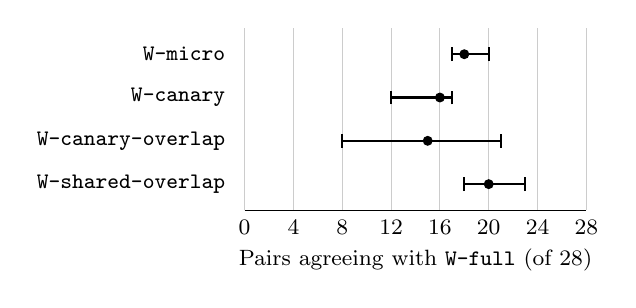
\begin{tikzpicture}[x=0.155cm,y=0.55cm,font=\footnotesize]
\draw[gray!40] (0,-0.6) -- (0,3.6);
\node[below] at (0,-0.6) {0};
\draw[gray!40] (4,-0.6) -- (4,3.6);
\node[below] at (4,-0.6) {4};
\draw[gray!40] (8,-0.6) -- (8,3.6);
\node[below] at (8,-0.6) {8};
\draw[gray!40] (12,-0.6) -- (12,3.6);
\node[below] at (12,-0.6) {12};
\draw[gray!40] (16,-0.6) -- (16,3.6);
\node[below] at (16,-0.6) {16};
\draw[gray!40] (20,-0.6) -- (20,3.6);
\node[below] at (20,-0.6) {20};
\draw[gray!40] (24,-0.6) -- (24,3.6);
\node[below] at (24,-0.6) {24};
\draw[gray!40] (28,-0.6) -- (28,3.6);
\node[below] at (28,-0.6) {28};
\draw (0,-0.6) -- (28,-0.6);
\node[anchor=east] at (-0.8,3) {\texttt{W-micro}};
\draw[line width=0.8pt] (17.0,3) -- (20.0,3);
\draw[line width=0.8pt] (17.0,2.84) -- (17.0,3.16);
\draw[line width=0.8pt] (20.0,2.84) -- (20.0,3.16);
\fill (18.0,3) circle (1.8pt);
\node[anchor=east] at (-0.8,2) {\texttt{W-canary}};
\draw[line width=0.8pt] (12.0,2) -- (17.0,2);
\draw[line width=0.8pt] (12.0,1.84) -- (12.0,2.16);
\draw[line width=0.8pt] (17.0,1.84) -- (17.0,2.16);
\fill (16.0,2) circle (1.8pt);
\node[anchor=east] at (-0.8,1) {\texttt{W-canary-overlap}};
\draw[line width=0.8pt] (8.0,1) -- (21.0,1);
\draw[line width=0.8pt] (8.0,0.84) -- (8.0,1.16);
\draw[line width=0.8pt] (21.0,0.84) -- (21.0,1.16);
\fill (15.0,1) circle (1.8pt);
\node[anchor=east] at (-0.8,0) {\texttt{W-shared-overlap}};
\draw[line width=0.8pt] (18.0,0) -- (23.0,0);
\draw[line width=0.8pt] (18.0,-0.16) -- (18.0,0.16);
\draw[line width=0.8pt] (23.0,-0.16) -- (23.0,0.16);
\fill (20.0,0) circle (1.8pt);
\node at (14,-1.75) {Pairs agreeing with \texttt{W-full} (of 28)};
\end{tikzpicture}

  \caption{Pairs on which each proxy agrees with the full workload. Dots are
  the measured counts; bars are 95\% repetition-bootstrap intervals. No proxy
  reaches 80\%, which is 22.4 pairs.}
  \label{fig:agreement}
\end{figure}

\subsection{Concurrency changes the ranking}

Adding overlap changes both pair agreement and tie structure.
\wname{canary-overlap} agrees on 15 of 28 pairs, or 53.6\%, while its
$\tau_b$ is 0.677. It never reverses a pair: all 13 of its disagreements are
pairs it labels a tie where \wname{full} does not. Its medians span only
144--178\,$\mu$s while cell IQRs reach 18\,$\mu$s, so the IQR tie rule
resolves few pairs. Its one-pair deficit against \wname{canary} is not resolved
by the bootstrap (interval $-7$ to $+6$). The disagreements concern ties rather
than reversed pairs.

\wname{shared-overlap} has the highest point agreement at 20 of 28 pairs,
or 71.4\%, with $\tau_b=0.708$. It agrees on more pairs than \wname{canary} in
99.9\% of bootstrap draws. Its two-pair lead over \wname{micro} is not resolved
(interval $-1$ to $+5$). Both overlap replays place the two low-latency (LL)
protocol configurations exactly where \wname{full} does, fifth and eighth,
while \wname{canary} places them first and second. Eight pair decisions still
disagree with \wname{full}; this comparison supplies no qualification verdict
for overlap replay.

\paragraph{Stability.} The trusted join applies no stability rule. Measured
against the exact-work gate's 20\% relative-IQR limit, every one of its 40
workload-configuration cells passes; the largest is 10.1\%, for
\texttt{nccl-2.20.5-tree-ll} under \wname{canary-overlap}. In \wname{full},
the same configuration has a relative IQR of 7.2\%, the widest of the eight but
within the limit. The 47.5\% instability reported for the gate in
Section~\ref{sec:verdict} belongs to that separate campaign's source
measurement.

The trusted join is descriptive and predates the separate exact-work policy.
We do not apply a new decision threshold after observing the result; the
intervals and exclusion analysis above qualify the reported counts rather than
turning them into a gate.

\subsection{The cost of the recommended configuration}

Table~\ref{tab:regret} reports the retrospective analysis. The reference's
lowest median is $8{,}203.264\us$ for \texttt{nccl-2.20.5-ring-ll128}.
Both \wname{micro} and \wname{canary} choose ring-LL and incur 3.16\% point
regret, although their agreement counts differ. The shared-overlap proxy has
the highest pair agreement, but chooses \texttt{nccl-2.19.3-default}, with
0.45\% point regret. Configuration-specific overlap has the lowest agreement
count yet chooses the reference optimum. Its first-choice interval extends
to 3.27\%, so zero point regret does not establish reliable optimal selection.

The shortlist results distinguish the proxies further. A
two-choice microbenchmark shortlist contains the reference optimum; the
communication-only shortlist still has 3.16\% regret and places the reference's
worst configuration second. Both overlap proxies place that configuration
last. Agreement, recommendation cost, and avoidance of the worst configuration
answer different questions. These results describe this finite decision set;
they neither rank proxies universally nor change the exact-work verdict.

\begin{table*}[t]
\caption{Retrospective decision regret on the retained trusted join. Lower
regret is better. $r_2$ and $r_3$ use the best reference result in each proxy's
shortlist. Intervals describe $r_1$ only. Worst rank is the proxy's position
for the full workload's slowest configuration (8 is last).}
\label{tab:regret}
\centering\small
% Generated by scripts/decision_regret.py; do not edit.
\begin{tabular}{@{}lrrrrr@{}}
\toprule
Proxy & $r_1$ (\%) & 95\% interval & $r_2$ (\%) & $r_3$ (\%) & Worst rank \\
\midrule
\wname{micro} & 3.16 & 2.06--4.48 & 0.00 & 0.00 & 6/8 \\
\wname{canary} & 3.16 & 2.06--4.48 & 3.16 & 0.45 & 2/8 \\
\wname{canary-overlap} & 0.00 & 0.00--3.27 & 0.00 & 0.00 & 8/8 \\
\wname{shared-overlap} & 0.45 & 0.07--0.72 & 0.34 & 0.34 & 8/8 \\
\bottomrule
\end{tabular}

\end{table*}

\subsection{Exact-work point estimates}

Exact work agrees on 26 of 28 pairs, or 92.86\%, with $\tau_b=0.857$. It
records one false negative and one false positive. Median absolute relative
error is 1.55\%, and p95 error is 4.05\%. It gains seven agreeing pairs over
the isolated control and sixteen over the stratified control. Every point
criterion passes, as Table~\ref{tab:criteria} records.

The gate also ran two ablations of exact work. Executing the same
compute and communication serialized, with no overlap, agrees on 18 of 28
pairs; removing rank arrival skew agrees on 24. Agreement therefore drops by
eight pairs when overlap is removed and by two when skew is removed. These
within-campaign comparisons support a role for concurrency in the measured
ranking. They are point counts; the gate did not compute intervals on them.

These estimates show that exact-work reconstruction is substantially closer to
the source ordering than the controls in this campaign. They do not determine
the final claim because a pair decision also requires a supported interval and
stable input measurements.

\begin{table*}[t]
\caption{Predeclared exact-work point criteria. Every point row passes, but the
final verdict also requires supported uncertainty and stability.}
\label{tab:criteria}
\centering\small
\begin{tabular}{@{}lrrc@{}}
\toprule
Criterion & Observed & Required & Point status \\
\midrule
Pair agreement & 92.86\% & at least 80\% & pass \\
Kendall $\tau_b$ & 0.857 & at least 0.7 & pass \\
False negatives & 1 & at most 1 & pass \\
False positives & 1 & at most 1 & pass \\
Median absolute relative error & 1.55\% & at most 10\% & pass \\
p95 absolute relative error & 4.05\% & at most 15\% & pass \\
Agreement advantage over isolated & 7 pairs & at least 2 pairs & pass \\
Agreement advantage over stratified & 16 pairs & at least 2 pairs & pass \\
\bottomrule
\end{tabular}
\end{table*}

\subsection{The verdict is inconclusive}
\label{sec:verdict}

The persisted outcome is \emph{inconclusive}. Two conditions prevent pass.

First, bootstrap intervals for several exact-work pair differences cross the
frozen decision regions. Figure~\ref{fig:inconclusive} normalizes representative
differences and 95\% intervals by each pair's tie threshold. An interval below
$-1$ supports the second configuration, an interval above $+1$ supports the
first, and an interval contained within $[-1,+1]$ supports a tie. Crossing
those regions leaves the label unsupported.

Second, \texttt{nccl-2.20.5-tree-ll} exceeds the 20\% relative-IQR limit in
source at 47.5\%, exact work at 32.3\%, and the stratified control at 50.4\%.
The source measurement itself therefore violates the stability requirement,
preventing qualification involving that configuration under the frozen policy.

Exact work agrees with more source decisions than the controls at the point
estimate. Its inconclusive verdict leaves decision preservation unqualified
under the frozen policy.

\begin{figure*}[t]
  \centering
  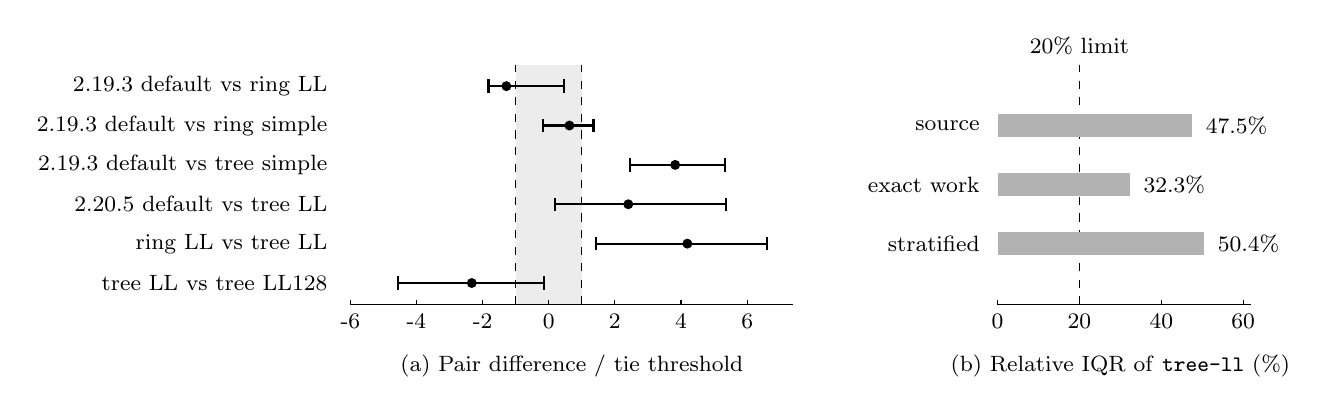
\begin{tikzpicture}[font=\footnotesize]
\begin{scope}[x=0.42cm,y=0.5cm]
\fill[gray!15] (-1,-0.55) rectangle (1,5.55);
\draw[dashed] (-1,-0.55) -- (-1,5.55);
\draw[dashed] (1,-0.55) -- (1,5.55);
\node[below] at (-6,-0.55) {-6};
\draw (-6,-0.55) -- (-6,-0.43);
\node[below] at (-4,-0.55) {-4};
\draw (-4,-0.55) -- (-4,-0.43);
\node[below] at (-2,-0.55) {-2};
\draw (-2,-0.55) -- (-2,-0.43);
\node[below] at (0,-0.55) {0};
\draw (0,-0.55) -- (0,-0.43);
\node[below] at (2,-0.55) {2};
\draw (2,-0.55) -- (2,-0.43);
\node[below] at (4,-0.55) {4};
\draw (4,-0.55) -- (4,-0.43);
\node[below] at (6,-0.55) {6};
\draw (6,-0.55) -- (6,-0.43);
\draw (-6,-0.55) -- (7.4,-0.55);
\node[anchor=east] at (-6.4,5) {2.19.3 default vs ring LL};
\draw[line width=0.8pt] (-1.8238,5) -- (0.4674,5);
\draw[line width=0.8pt] (-1.8238,4.83) -- (-1.8238,5.17);
\draw[line width=0.8pt] (0.4674,4.83) -- (0.4674,5.17);
\fill (-1.2797,5) circle (1.8pt);
\node[anchor=east] at (-6.4,4) {2.19.3 default vs ring simple};
\draw[line width=0.8pt] (-0.1728,4) -- (1.3540,4);
\draw[line width=0.8pt] (-0.1728,3.83) -- (-0.1728,4.17);
\draw[line width=0.8pt] (1.3540,3.83) -- (1.3540,4.17);
\fill (0.6266,4) circle (1.8pt);
\node[anchor=east] at (-6.4,3) {2.19.3 default vs tree simple};
\draw[line width=0.8pt] (2.4487,3) -- (5.3367,3);
\draw[line width=0.8pt] (2.4487,2.83) -- (2.4487,3.17);
\draw[line width=0.8pt] (5.3367,2.83) -- (5.3367,3.17);
\fill (3.8243,3) circle (1.8pt);
\node[anchor=east] at (-6.4,2) {2.20.5 default vs tree LL};
\draw[line width=0.8pt] (0.1916,2) -- (5.3701,2);
\draw[line width=0.8pt] (0.1916,1.83) -- (0.1916,2.17);
\draw[line width=0.8pt] (5.3701,1.83) -- (5.3701,2.17);
\fill (2.4060,2) circle (1.8pt);
\node[anchor=east] at (-6.4,1) {ring LL vs tree LL};
\draw[line width=0.8pt] (1.4320,1) -- (6.5927,1);
\draw[line width=0.8pt] (1.4320,0.83) -- (1.4320,1.17);
\draw[line width=0.8pt] (6.5927,0.83) -- (6.5927,1.17);
\fill (4.1916,1) circle (1.8pt);
\node[anchor=east] at (-6.4,0) {tree LL vs tree LL128};
\draw[line width=0.8pt] (-4.5649,0) -- (-0.1344,0);
\draw[line width=0.8pt] (-4.5649,-0.17) -- (-4.5649,0.17);
\draw[line width=0.8pt] (-0.1344,-0.17) -- (-0.1344,0.17);
\fill (-2.3267,0) circle (1.8pt);
\node at (0.7,-2.1) {(a) Pair difference / tie threshold};
\end{scope}
\begin{scope}[xshift=5.7cm,x=0.052cm,y=0.5cm]
\draw (0,-0.55) -- (62,-0.55);
\node[below] at (0,-0.55) {0};
\draw (0,-0.55) -- (0,-0.43);
\node[below] at (20,-0.55) {20};
\draw (20,-0.55) -- (20,-0.43);
\node[below] at (40,-0.55) {40};
\draw (40,-0.55) -- (40,-0.43);
\node[below] at (60,-0.55) {60};
\draw (60,-0.55) -- (60,-0.43);
\draw[dashed] (20,-0.55) -- (20,5.55);
\node[anchor=south] at (20,5.55) {20\% limit};
\node[anchor=east] at (-2,4.0) {source};
\fill[gray!60] (0,3.70) rectangle (47.4731,4.30);
\node[anchor=west] at (48.4731,4.0) {47.5\%};
\node[anchor=east] at (-2,2.5) {exact work};
\fill[gray!60] (0,2.20) rectangle (32.2775,2.80);
\node[anchor=west] at (33.2775,2.5) {32.3\%};
\node[anchor=east] at (-2,1.0) {stratified};
\fill[gray!60] (0,0.70) rectangle (50.4286,1.30);
\node[anchor=west] at (51.4286,1.0) {50.4\%};
\node at (30,-2.1) {(b) Relative IQR of \texttt{tree-ll} (\%)};
\end{scope}
\end{tikzpicture}

  \caption{Why the exact-work verdict is inconclusive. (a) Representative
  pair differences with 95\% bootstrap intervals, in units of each pair's tie
  threshold; an interval spanning a boundary of the shaded tie band does not
  support a unique label. (b) \texttt{nccl-2.20.5-tree-ll} exceeds the frozen
  20\% stability limit in three representations.}
  \label{fig:inconclusive}
\end{figure*}

\subsection{Same-node diagnostic}

A separate one-cell diagnostic compares retained source and replay timing for
one exact-work capsule. The source median is $1{,}434.1\us$ and the replay
median is $1{,}541.0\us$, a signed difference of $+106.9\us$, or $+7.45\%$. All 32 deterministic checks pass across four ranks.
Table~\ref{tab:diagnostic} summarizes the diagnostic.

The diagnostic confirms deterministic reconstruction checks and a same-node
timing comparison. It has no multi-configuration full-workload matrix. It
cannot issue a qualification verdict or substitute for the inconclusive
decision gate.

\begin{table}[t]
\caption{Exact-work diagnostic. No qualification verdict is issued.}
\label{tab:diagnostic}
\centering\small
\begin{tabularx}{\columnwidth}{@{}lY@{}}
\toprule
Item & Result \\
\midrule
Source median & $1{,}434.1\us$ \\
Replay median & $1{,}541.0\us$ \\
Signed difference & $+106.9\us$ ($+7.45\%$) \\
Source / replay IQR & $9.2 / 9.0\us$ \\
Deterministic checks & 32 passed across 4 ranks \\
Claim status & diagnostic; physical fidelity unproven; verdict not issued \\
\bottomrule
\end{tabularx}
\end{table}

\section{Interpretation}

\subsection{A trace encodes a causal hypothesis}

A communication trace selects the workload properties assumed to determine
the configuration choice. The communication-only representation assumes that
collective type, size, order, and synchronization are sufficient. The trusted
join rejects that assumption for the measured case. The operation stream can
be faithful at the communication interface while omitting concurrent work that
changes endpoint contention and critical-path timing.

The overlap results help explain the disagreements. The configuration-specific
overlap replay has fewer exact pair matches than the microbenchmark, but all
of its mismatches are ties rather than reversed pairs. The shared-trace variant,
which holds replayed work constant across configurations, has the highest
point agreement. Together with the exact-work ablation, these observations
indicate that concurrency affects the measured ranking. They do not establish
that adding overlap alone is sufficient to preserve it.

\subsection{A hypothesis for the mechanism}

Both misplaced configurations use NCCL's LL protocol, which transfers data
with flags that the receiving kernel polls~\cite{nccl}. We hypothesize that
these transfers contend with concurrent GEMM work for streaming multiprocessor
and memory resources, reducing the advantage seen without compute. The
observed rankings are consistent with this explanation but do not identify
the contended resource. With compute removed,
\wname{micro} and \wname{canary} rank ring-LL first; in \wname{full} it is
fifth. \wname{canary} ranks tree-LL second; in \wname{full} it is last, 38\%
behind the fastest configuration, with the widest spread of the eight. Both
overlap replays, which restore concurrent compute, put the two LL
configurations exactly where \wname{full} does. The gate's overlap ablation
points the same way within one campaign.

The larger tree-LL displacement in \wname{canary} than in \wname{micro} is
also unexplained. Both omit compute; \wname{canary} replays the recorded
asynchronous requests and explicit waits, while \wname{micro} issues blocking calls back to
back. A replay that keeps several requests in flight may reward a
latency-optimized protocol further, but this hypothesis has not been tested.
Measuring GEMM slowdown and collective time per configuration under controlled concurrency,
and repeating the comparison with NCCL channel counts fixed, would test both
hypotheses.

\subsection{Decision versus timing fidelity}

Absolute error and decision fidelity can diverge. Two configurations may differ
by less than measurement variability. A replay can have small percentage error
and reverse them, or a common timing bias and preserve their order. We report
pair labels, rank correlation, false-negative and false-positive counts, and
timing errors separately.

In the exact-work experiment, low median and p95 errors satisfy the timing
criteria, but each operational decision must also be supported under
uncertainty. A 92.86\% point agreement is not a 92.86\% probability that
the replay is correct. An interval that crosses a decision boundary leaves
the point label unsupported.

\subsection{Fail-closed evidence as the default}

Experiment scripts often make it easy to produce a number. Missing runs can
disappear during aggregation, and retries can overwrite failures. A fail-closed
path makes incompleteness visible, preserves failed attempts, and requires
explicit selection before analysis. It adds operational work and metadata, but
it lets a later reader distinguish a complete negative result from an
incomplete favorable subset.

The exact-work verdict is the direct example. A threshold-only summary would
report that every numeric row passed. Because uncertainty and stability are
policy conditions, the retained conclusion is inconclusive.

\subsection{Scope of the evidence}

The evidence does not show that communication-only replay is generally worse
than a microbenchmark; that ordering depends on one configuration. It does not
show that a reduced physical canary is cheaper than the full workload. Replay proxies are not a completed product corpus, and no
held-out physical regression study is present. The checked-in publication
package has no real vLLM or SGLang application campaign. Exact work is a
positive reconstruction control, not evidence that minimization succeeded.

The negative result is limited to configuration decisions in the measured
single-node, four-A100 matrix. Communication-only replay can still support
debugging, transport isolation, or reproduction of a call sequence without
preserving a workload's configuration ranking.

\section{Threats to validity}

\paragraph{Single system and workload.} All physical data come from one
four-A100 PCIe node and one source-derived workload family. GPU topology, CPU
placement, software versions, thermal state, and site configuration may affect
the ranking. The result does not generalize to multi-node systems, NVSwitch,
other GPU generations, or vendor qualification.

\paragraph{Finite configuration set.} The decision object contains eight NCCL
configurations. It does not cover every environment variable, channel count,
topology override, message size, or collective library. Adding configurations
changes the number and difficulty of pair decisions.

\paragraph{Tie-policy sensitivity.} The trusted join uses an IQR rule. The
exact-work gate uses a pair-specific absolute or relative band with bootstrap
uncertainty. Both policies were frozen for their experiments, but another
operational tie definition could change labels. Exact counts and $\tau_b$ are
reported so the effect remains visible.

\paragraph{Uncertainty in the trusted join.} Each trusted-join cell has five
selected repetitions. The repetition bootstrap may understate uncertainty,
and the full-workload labels themselves move: six of the 28
reference pair labels keep their point value in fewer than 95\% of draws. The
proxy comparisons are reported with both their intervals and tree-LL
sensitivity. The regret analysis reuses these observations and is not an
independent replication. Its intervals do not establish a general ordering
between proxies.

\paragraph{Measurement dependence.} Repeated timings within one process may be
dependent. The independent percentile bootstrap is a predeclared approximation,
not a universal model of system noise. A block or hierarchical bootstrap may
be preferable when temporal dependence is strong. Replication across nodes and
days remains future work.

\paragraph{Shared implementation.} A defect shared by source capture,
materialization, and verification could evade deterministic checks. Hash
binding proves byte identity, not semantic correctness. Independent producers,
differential implementations, and application invariants would provide
stronger controls.

\paragraph{Researcher choices.} Explicit selection and completeness reduce
post-hoc cell dropping, but campaign design, configuration choice, and policy
thresholds remain researcher decisions. The exact-work gate freezes thresholds
before analysis. The trusted join is a measured comparison, not a formal gate
defined after the result.

\paragraph{Publication boundary.} The paper uses generated artifacts retained
at a specific evidence commit. Older narrative measurements without complete
evidence are excluded. This avoids unsupported reuse, although it omits
historical observations that cannot now be independently reconstructed.

\section{Artifact availability}

The source repository is available at
\url{https://github.com/iemAnshuman/CommCanary}. Every physical number in this
paper comes from evidence already present at commit
\begin{center}
\texttt{c133ad3fb5883100cb8622b597d5b6233b5efca1}.
\end{center}
Implementation descriptions and the decision-regret scorer are bound to
\href{https://github.com/iemAnshuman/CommCanary/tree/cefad5a086b4723755bbe33b33e96f9f3a2c8e36}{commit \texttt{cefad5a086b47}}.
The revision adds analysis of retained observations, not new hardware
measurements. An earlier version of this work is archived under the concept DOI
\href{https://doi.org/10.5281/zenodo.21939040}{10.5281/zenodo.21939040}.

Campaigns retain their own manifest, selection, completeness, archive, and
repository identities. The outer evidence commit and source tree used to
prepare the paper are separate states. The per-attempt raw evidence of every
campaign used here is committed at the evidence commit as normalized,
hash-described archives stored with Git LFS; a clone must run
\texttt{git lfs pull}. The trusted-join aggregate was generated before those
archives were bound and records its raw archive as unverified. Regenerating it
therefore first restores each campaign's selected workspace files from its
archive, about 9\,GB uncompressed for the three campaigns, with
\texttt{python -m experiments.rostam.restore\_workspaces}, then runs the
regeneration command recorded in the aggregate. The trusted join is under
\path{experiments/rostam/results/publications/}. The exact-work diagnostic is
under \path{experiments/rostam/results/exact-work-artifacts/publication/}.
The authoritative directory names are:

\begin{itemize}
  \item \texttt{trusted-join-core-}\allowbreak
    \texttt{shared-overlap-primary/};
  \item \texttt{decision-gate-20260801-r3-}\allowbreak
    \texttt{analysis-1300d12-primary/};
  \item the corresponding reproduction directory; and
  \item \path{qualification-exact-20260730-r3-primary/}.
\end{itemize}

The supplied scripts regenerate every vector figure from
\texttt{evidence/verified\_metrics.json} and every interval and sensitivity
value from \texttt{evidence/trusted\_join\_uncertainty.json}, which
\texttt{scripts/trusted\_join\_uncertainty.py} rebuilds from the committed
aggregate. That compact snapshot records verified
values and their paper binding.
\texttt{scripts/decision\_regret.py} verifies the retained aggregate hashes
and emits \texttt{evidence/decision\_regret.json} and the corresponding
LaTeX table; its \texttt{--check} mode requires exact regeneration of both.
The JSON includes the five measurement sets and all bootstrap settings.
These files do not replace immutable result
directories. Reproducing physical timings still requires recorded hardware and
software; deterministic analysis does not imply hardware-independent
measurements.

\section{Related work}

\paragraph{Collective algorithms and tuning.} MPI defines collective semantics
but leaves the algorithm to the implementation~\cite{mpi}. MPICH studies show
why message size and process count affect algorithm selection~\cite{thakur}.
Performance models seek to predict or tune these choices~\cite{vadhiyar}. NCCL
provides GPU collectives and configurable algorithms and protocols~\cite{nccl};
NCCL Tests supplies operation-level measurements~\cite{nccltests}. CommCanary
uses the full-workload decision as the reference and tests whether a trace
representation preserves it.

\paragraph{Trace representation and replay.} ScalaTrace retains replay
capability while compressing communication traces~\cite{scalatrace}.
LogGOPSim simulates trace-driven communication at scale~\cite{loggopsim}.
ASTRA-SIM models distributed-learning workloads and networks
\cite{astrasim,astrasim2}. Chakra provides an execution-trace graph, Mystique
derives portable benchmarks from execution traces, and PARAM provides benchmark
and replay machinery~\cite{chakra,mystique,param}. CommCanary focuses on a
failure mode that these representations do not remove: a valid communication
trace can still change the configuration decision when it omits causal workload
context.

\paragraph{Compute and communication concurrency.} Earlier work measures the
resource interaction between computation and collective communication and
develops overlap mechanisms~\cite{overlap}. CommCanary does not introduce
another overlap engine. The experiments show that removing or changing overlap
alters which NCCL configuration appears preferable in the measured case.

\paragraph{Reduction and workload minimization.} Delta debugging removes input
while preserving a predicate~\cite{ddmin}. CommCanary implements experimental
predicate-based and phase-representative reduction, and dependency-closed
physical candidate selection (Section~\ref{sec:implementation}). The
publication evidence contains no completed reduced physical canary or cost
result. Implemented selection methods therefore remain unqualified for
physical decision preservation.

\paragraph{Statistical comparison.} Benchmarking guidance warns against
selective statistics and incomplete variability reports~\cite{benchmarking}.
We pair exact decisions with Kendall's statistic~\cite{kendall} and use a
predeclared bootstrap procedure~\cite{efron}. Uncertainty and stability are
verdict conditions instead of annotations added after a point estimate.

\section{Conclusion}

The 280-cell comparison shows that communication-only replay changes the
configuration ranking on the measured single-node, four-A100 system.
\wname{canary} reaches
57.1\% pair agreement and ranks the full workload's slowest configuration
second. Replay that keeps compute concurrent with communication places the
low-latency-protocol configurations where the full workload does; the
highest pair agreement among these replays is 71.4\%, leaving eight
disagreements. The reported difference intervals all include zero when tree-LL
is excluded. Retrospective regret measures a different consequence:
the proxy with the fewest agreeing pairs chooses the measured optimum, while
communication-only replay and the microbenchmark incur 3.16\% point regret.

Exact work agrees with more source decisions than either control. Its 92.86\%
agreement, $\tau_b=0.857$, and low relative errors pass every point threshold. The final
outcome remains inconclusive because pair uncertainty crosses decision
boundaries and one configuration violates the stability limit.

The supported contribution is an independently verifiable, fail-closed
evidence workflow and a measured result about the role of concurrency.
Production qualification, reduced-canary savings, held-out regression safety,
application product studies, and generalization beyond the measured system
remain open.

\bibliographystyle{unsrt}
\bibliography{references}

\clearpage
\onecolumn
\appendix
\section{Campaign identities}

Table~\ref{tab:identities} lists abbreviated campaign identities. Full SHA-256
values remain in \texttt{evidence/verified\_metrics.json} and authoritative
repository artifacts.

\begin{table}[htbp]
\caption{Abbreviated manifest-bound campaign identities (first 12 hex digits).}
\label{tab:identities}
\centering\small
\begin{tabular}{@{}lllll@{}}
\toprule
Run & Manifest & Selection & Completeness & Repository \\
\midrule
\texttt{core-20260724-r7} & \texttt{3bd321ec960c} & \texttt{d01db822c8e9} & \texttt{46d8012b3594} & \texttt{2855275288e6} \\
\texttt{shared-replay-20260720-r2} & \texttt{a402a4ec73ea} & \texttt{a1e876861f7f} & \texttt{b6cd1aae4cfb} & \texttt{2855275288e6} \\
\texttt{overlap-20260724-r1} & \texttt{5d5eb9f4822e} & \texttt{e012e40613f5} & \texttt{5b153d0452df} & \texttt{2855275288e6} \\
\texttt{decision-gate-20260801-r3} & \texttt{1b1909b3e856} & \texttt{c675e42e34e4} & \texttt{6377a65bb057} & \texttt{4585318ac244} \\
\texttt{qualification-exact-20260730-r3} & \texttt{c0bc2e6a9ecb} & \texttt{bf23480f39dd} & \texttt{593772c09020} & \texttt{9b1e58aef91e} \\
\bottomrule
\end{tabular}
\end{table}

\section{Trusted-join regeneration}

The generated publication fragment retains the analyzer invocation with its
exact argument order. The complete command is included in the source package
at \texttt{evidence/trusted\_join\_regeneration.txt}. It binds the core
campaign, primary selection and completeness verdict, joined evidence
directories, output directory, configuration identities, and median
thresholds.

\end{document}
